\documentclass[11pt,a4paper]{article}
\usepackage[T1]{fontenc}
\usepackage[utf8]{inputenc}
\usepackage{lmodern,microtype}
\usepackage[margin=23mm]{geometry}
\usepackage{amsmath,amssymb,booktabs,graphicx,array}
\usepackage{siunitx,tikz}
\usetikzlibrary{arrows.meta,decorations.pathreplacing}
\usepackage[numbers,sort&compress]{natbib}
\usepackage[colorlinks=true,linkcolor=blue!45!black,citecolor=blue!45!black,urlcolor=blue!45!black]{hyperref}
\IfFileExists{../../latex_generated/ion_readout/csa_design/values.tex}{\def\CsaGenerated{../../latex_generated/ion_readout/csa_design/}}{\def\CsaGenerated{./}}
\graphicspath{{\CsaGenerated}{figures/}{../../notes/physics/figures/}}
\input{\CsaGenerated values.tex}
\newcommand{\dd}{\mathrm{d}}
\newcommand{\sinc}{\operatorname{sinc}}
\setlength{\parindent}{0pt}
\setlength{\parskip}{5pt plus 1pt}
\setlength{\emergencystretch}{2em}
\title{NAUSICAA CSA: design, readout and response to ion tracks}
\author{J. J. G\'omez-Cadenas \quad Vicente Herrero \quad Rogelio Palomo}
\date{\today}
\begin{document}
\maketitle

\begin{abstract}
This note describes the working design of the NAUSICAA charge-sensitive amplifier
and the calculation used to reconstruct ions arriving in successive readout
frames. A slow feedback discharge, nominally \SI{\CsaNominalTau}{s}, and voltage
averages over \SI{\CsaAverageMs}{ms} give a reconstructed frame noise of
\CsaEncTwo--\CsaEncFour\ elementary charges RMS. Complete pad histories are used to calculate accumulated
voltage, compression and noise. Pilot samples compare 2, 3 and 4 mm pad pitches
with 20, 30 and 40 ms frames. The reconstructed ion matrices are saved for the
track analysis.
\end{abstract}

\section{The working circuit}

Each metal pad is connected to a charge-sensitive amplifier (CSA). The ion
current changes the charge on the feedback capacitor $C_f$ and therefore the
output voltage. Negative feedback keeps the input voltage nearly constant.
With sufficient amplifier gain, an input charge $Q$ changes the output by
approximately $-Q/C_f$. The transistor calculation determines the actual
response, including finite gain, bandwidth and feedback discharge.

Figure~\ref{fig:circuit} shows the circuit. The pad drives the gate of the PMOS
input transistor $M_1$. A change in its gate voltage changes its current. The
$M_2$ and $M_3$ branch establishes the input-stage operating point; $M_4$ carries
the signal into the output branch, whose PMOS load is formed by $M_5$ and $M_6$.
The output is connected back to the input through $C_f$ and $M_f$.
The capacitance integrates charge. The small current through $M_f$ restores the
baseline continuously.

\begin{figure}[htbp]
\centering
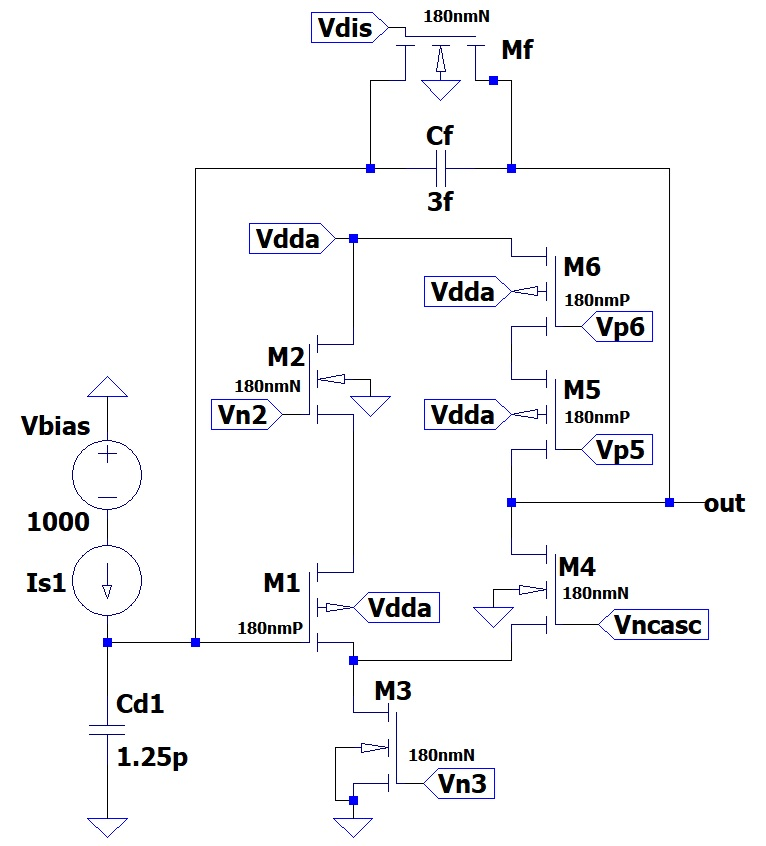
\includegraphics[width=.70\linewidth]{Nausica_Image.jpg}
\caption{CSA topology supplied by Rogelio Palomo. The input source represents
the pad current. The external input capacitance is $C_{\rm ext}$; the transistor
models add their own capacitances. Device dimensions and operating voltages
used in the calculation are given in Tables~\ref{tab:devices} and~\ref{tab:bias}.}
\label{fig:circuit}
\end{figure}

The circuit uses 180 nm CMOS models, a supply of \SI{\CsaSupply}{V},
$C_f=\SI{\CsaCfFf}{fF}$ and an external input capacitance
$C_{\rm ext}=\SI{\CsaCinPf}{pF}$. This external value is a design input held fixed
throughout the comparison. The simulated temperature is
\SI{\CsaTemperature}{K}. At the quiescent operating point the output is
\SI{\CsaBaseline}{V}, the supply current is \SI{\CsaCurrentUa}{\micro\ampere}
and the corresponding circuit power is \SI{\CsaPowerMw}{mW} per channel.

\begin{table}[htbp]\centering
\caption{Transistor dimensions from the simulated v3 netlist. Multiplicity
counts parallel devices with the listed dimensions.}
\label{tab:devices}
\input{\CsaGenerated transistors.tex}
\end{table}
\begin{table}[htbp]\centering
\caption{Bias voltages, rounded for display. The saved netlists retain the
values used in the simulation.}
\label{tab:bias}
\input{\CsaGenerated biases.tex}
\end{table}

\section{Why the feedback discharge is slow}

The input current from one ion is short. A pad can collect many ions over a
much longer interval, and its CSA integrates their currents continuously.
Between arrivals the feedback transistor removes some of the accumulated
charge. Its conductance therefore affects both signal retention and noise.

The selected feedback device has a long, narrow channel. Near the operating
point its current is very small, producing a slow return to baseline. The
small-signal tail is fitted by
\begin{equation}
 V(t)-V_0=B\exp(-t/\tau_f).
 \label{eq:tail}
\end{equation}
The fit gives $\tau_f=\SI{\CsaFittedTau}{s}$; the working design is labelled
``\SI{\CsaNominalTau}{s} retention''. This is a fitted property of the transistor
circuit. Its response at large accumulated voltage is calculated directly in
SPICE.

Figure~\ref{fig:retention} shows the retention scan. Increasing the feedback
length reduces its contribution to the filtered noise. The improvement becomes
smaller beyond the selected point. A longer discharge time also retains more
charge from earlier buckets, increasing the accumulated voltage. The full pad
histories are needed to check the resulting compression.

A retention time of \SI{\CsaNominalTau}{s} does not set the duration of a readout
frame. Voltage readings continue throughout the event, at intervals of 20,
30 or 40 ms. The signal from earlier charge is accounted for when differences
between readings are converted into bucket counts.

\begin{figure}[htbp]\centering
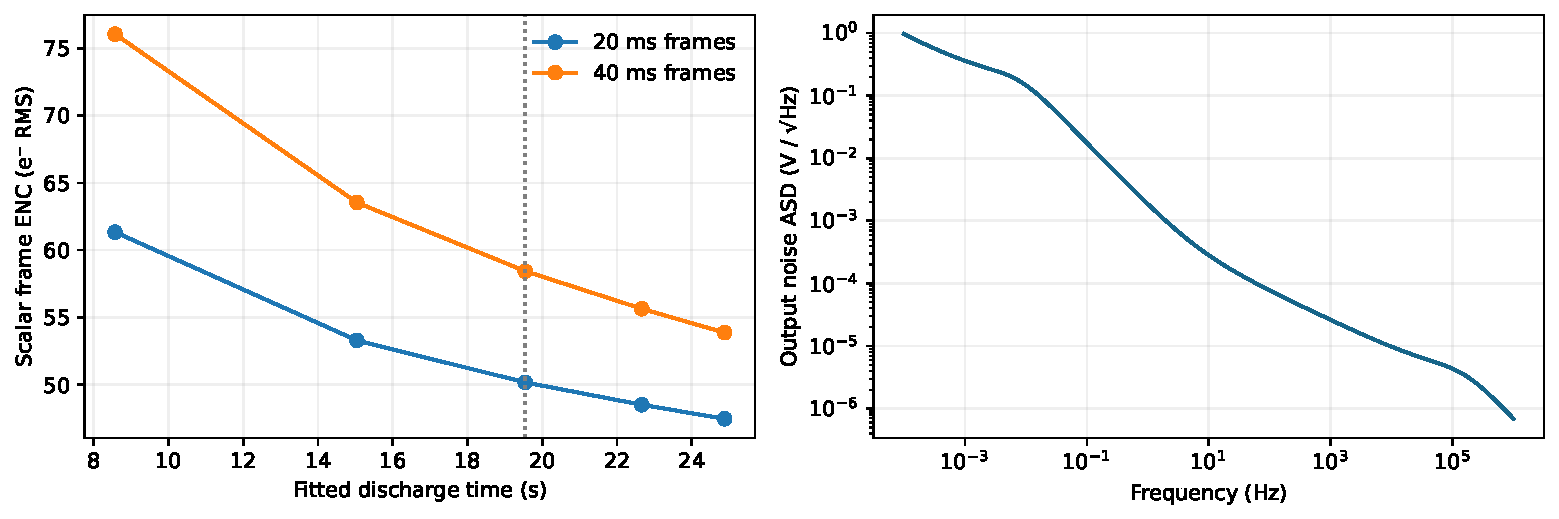
\includegraphics[width=\linewidth]{retention_noise.pdf}
\caption{Left: the saved retention scan, with 5 ms averaging and a
feedback-corrected frame difference. These ENC values precede the three-frame
reconstruction described below. Each point uses its fitted discharge time and
its own operating-point calibration. The vertical line marks the selected
circuit. Right: its one-sided output noise amplitude spectral density from
SPICE.}
\label{fig:retention}
\end{figure}

\section{From bucket counts to the pad current}

The detector simulation supplies $N_{p,n}$, the number of positive ions
collected by pixel $p$ in bucket $n$. Each xenon molecular ion,
$\mathrm{Xe}_2^+$, carries charge $+e$. A bucket is an interval of collection
times. For this calculation the arrivals are distributed uniformly within it.

The current from one ion follows from the weighting potential
$\phi_w$~\cite{riegler2016}. This potential is calculated without free charge,
with the selected pad at unit potential and the other conductors at zero.
For the benchmark used here, the pad is a square of side
\SI{\CsaPadMm}{mm} in an infinite grounded plane. The gas is homogeneous above
the plane and the potential tends to zero at infinity. On the central axis,
for pad half-width $a$,
\begin{equation}
 W(z)=-\frac{\dd\phi_w}{\dd z}
 =\frac{4a^2}{\pi(z^2+a^2)\sqrt{z^2+2a^2}}.
 \label{eq:weight}
\end{equation}
This expression follows from the solid-angle potential of a square electrode;
its derivation is recorded in the single-ion appendix of
\texttt{notes/physics/nausica.tex}, using Ref.~\cite{salazar2021}.

Take collection at $t=0$. The ion approaches the centre at a constant speed
$v=\SI{\CsaGapSpeed}{m/s}$ through the final gap
$g=\SI{\CsaGapMm}{mm}$. With positive current delivered into the input,
\begin{equation}
 i_1(t)=evW(-vt),\qquad -g/v\leq t<0,
 \qquad
 \int i_1(t)\,\dd t=Q_g=e[1-\phi_w(g)].
 \label{eq:input}
\end{equation}
The finite-path integral is retained. Collection ends the current.
The actual IFG and surface dielectrics require a more detailed weighting-field
calculation; the present geometry fixes the input-current benchmark for all
three pilots.

For frame boundaries $t_n$, width $T=t_n-t_{n-1}$, and uniform mean arrival
times, the input to the circuit is
\begin{equation}
 i_p(t)=\sum_n\frac{N_{p,n}}{T}
       \int_{t_{n-1}}^{t_n}i_1(t-u)\,\dd u.
 \label{eq:history_current}
\end{equation}
The integration variable $u$ is the collection time. Thus induction can begin
before the bucket in which the ion reaches the pad. Consecutive buckets drive
one continuous transient, including the zero-ion buckets between deposits.

\section{Voltage readings and charge reconstruction}
\label{sec:readout}

\subsection{Averaging and frame differences}

Let $V(t)$ be the CSA output relative to its quiescent baseline. At each frame
boundary $t_n$, the readout uses the voltage averaged over a centred window of
width $T_a=\SI{\CsaAverageMs}{ms}$:
\begin{equation}
 \overline V_n=\frac{1}{T_a}
 \int_{t_n-T_a/2}^{t_n+T_a/2}V(t)\,\dd t.
 \label{eq:average}
\end{equation}
A physical readout can form this mean from repeated voltage samples over the
window. The present calculation performs the average on the SPICE transient.
Figure~\ref{fig:windows} shows its timing.

\begin{figure}[htbp]\centering
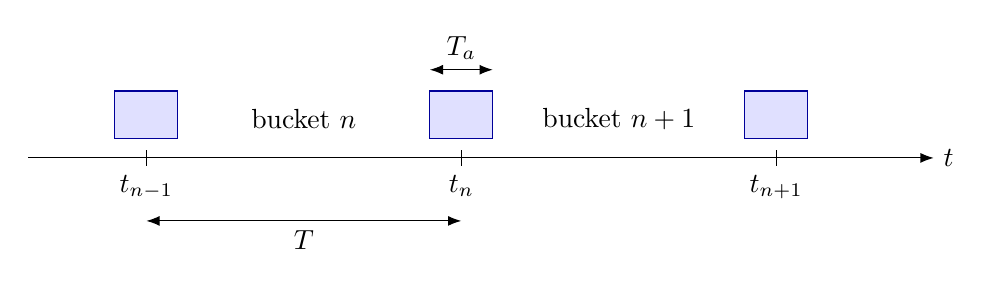
\begin{tikzpicture}[x=1.0cm,y=1cm,>=Latex]
 \draw[->] (-.5,0)--(11,0) node[right] {$t$};
 \foreach \x/\lab in {1/{t_{n-1}},5/{t_n},9/{t_{n+1}}}{
  \fill[blue!12] (\x-.4,.25) rectangle (\x+.4,.85);
  \draw[blue!60!black] (\x-.4,.25) rectangle (\x+.4,.85);
  \draw (\x,.1)--(\x,-.1) node[below] {$\lab$};
 }
 \draw[<->] (1,-.8)--(5,-.8) node[midway,below] {$T$};
 \draw[<->] (4.6,1.12)--(5.4,1.12) node[midway,above] {$T_a$};
 \node at (3,.5) {bucket $n$};\node at (7,.5) {bucket $n+1$};
\end{tikzpicture}
\caption{Voltage-averaging windows at successive frame boundaries. An average
combines samples within each shaded window. The difference uses two adjacent
averages. The drawing is schematic.}
\label{fig:windows}
\end{figure}

Earlier charge leaves a voltage that decays between boundaries. Define
$\alpha=\exp(-T/\tau_f)$. The measured frame difference is
\begin{equation}
 d_n=-(\overline V_n-\alpha\overline V_{n-1}),\qquad
 y_n=\frac{d_n}{g}.
 \label{eq:scalar}
\end{equation}
Here $g$, in volts per ion, is obtained from the SPICE response to a uniform
packet in one frame: it is that packet's central-frame $d_n$ divided by its
ion count. The sign makes positive ion charge give positive $y_n$.

For an ideal, rapidly responding CSA and negligible decay, the output is a
step for an instantaneous charge input. Averaging that step over $T_a$ gives
a ramp. The difference between two such ramps gives a trapezoidal charge
weight: a rising edge, a flat interval and a falling edge. Thus averaging and
frame differencing provide the shaping used in this calculation. The finite
circuit response and $\alpha$ determine its calibrated form.

\subsection{Removing contributions from neighbouring frames}

A centred averaging window overlaps both sides of a frame boundary. Induction
also starts before collection, and the amplifier takes time to respond.
Consequently a packet contributes to neighbouring $y_n$ values. Calibrating
only its central value leaves a positive bias when all frames are summed.

The saved small-signal packet response supplies three coefficients,
\begin{equation}
 y_n=b_{\rm late}N_{n-1}+N_n+b_{\rm early}N_{n+1}.
 \label{eq:taps}
\end{equation}
The central coefficient is one by the definition of $g$.
The coefficient $b_{\rm late}$ describes the response left by charge collected
in the preceding frame; $b_{\rm early}$ describes the response before charge
is collected in the following frame. Their numerical values and the longer
tail are checked against the saved circuit response.

Write Eq.~\eqref{eq:taps} as $\mathbf y=M\mathbf N$, with a tridiagonal $M$.
The reconstructed counts are
\begin{equation}
 \widehat{\mathbf N}=M^{-1}\mathbf y.
 \label{eq:inverse}
\end{equation}
The same solve is applied to the mean signal and the sampled noise. It removes
the linear frame mixing while retaining compression in the transistor
response. The saved interval includes \CsaQuietFrames\ quiet frames before the event
and \SI{\CsaRecoveryS}{s} of recovery afterwards. These quiet frames provide the
boundary conditions. Signed estimates are kept, including negative noise fluctuations.

\section{Noise in the reconstructed counts}

The transistor models supply thermal and flicker noise. Flicker noise becomes
larger towards low frequency, with a power spectrum approximately proportional
to $1/f$. SPICE propagates these device sources through the circuit and gives
the total output spectrum at the quiescent operating point. Let $S_V(f)$ be its
one-sided power spectral density, in $\mathrm{V^2/Hz}$.

The average and frame difference in Eqs.~\eqref{eq:average} and~\eqref{eq:scalar}
give the squared voltage weighting
\begin{equation}
 |F(f)|^2=
 \underbrace{\left[\frac{\sin(\pi fT_a)}{\pi fT_a}\right]^2}_{\text{average}}
 \underbrace{\left[(1-\alpha)^2+4\alpha\sin^2(\pi fT)\right]}_{\text{frame difference}}.
 \label{eq:filter}
\end{equation}
High-frequency fluctuations are reduced by averaging. Slowly varying offsets
largely cancel in the difference. Both operations must be included when noise
is compared with the measured ion signal.

The covariance of the scalar ion estimates, for integer frame lag $\ell$, is
\begin{equation}
 C_y(\ell)=\frac{1}{g^2}
 \int_{f_{\min}}^{f_{\max}}S_V(f)|F(f)|^2
       \cos(2\pi f\ell T)\,\dd f,
 \label{eq:covariance}
\end{equation}
with $f_{\min}=\SI{\CsaNoiseLow}{Hz}$ and
$f_{\max}=\SI{\CsaNoiseHighMHz}{MHz}$.
The covariance after reconstruction is
\begin{equation}
 C_{\widehat N}=M^{-1}C_yM^{-T},\qquad
 \mathrm{ENC}_n=\sqrt{(C_{\widehat N})_{nn}}.
 \label{eq:enc}
\end{equation}
The counts are expressed in elementary-charge units, so this standard
deviation is the equivalent noise charge (ENC), in electrons RMS.
Equation~\eqref{eq:covariance} and its numerical quadrature are implemented in
\texttt{bucket\_noise\_covariance.jl}; the inverse and covariance transformation
are implemented in \texttt{ion\_csa\_correction.jl}.

\begin{table}[htbp]\centering\small
\caption{Calibration from the selected circuit. $g$ converts the scalar frame
difference into ion counts. ENC$_y$ precedes the inverse and
ENC$_{\widehat N}$ follows it. $r_1$ is the interior lag-one correlation after
reconstruction. ENC values are in elementary charges RMS.}
\label{tab:calibration}
\input{\CsaGenerated calibration.tex}
\end{table}

The quoted ENC is the interior-frame value. The exact covariance for each
saved history includes its boundary frames. Gaussian noise is sampled with
this covariance, independently for each pad. A stable per-pad seed makes the
realisation reproducible. The stationary operating-point noise spectrum is
used for every mean history, including histories with compression.

\section{Pilot comparison}

Each configuration uses the same 100 deterministically spaced event IDs from
each sample of 8000 double-beta and 8000 single-electron events. The three
configurations share the sampled primary ionisation and event placement.
Changing pitch also changes the bucket duration: 2, 3 and 4 mm correspond to
20, 30 and 40 ms. Their effects are therefore compared together.

Every pad first receives a calibrated linear response. Direct SPICE transients
replace it where large accumulated voltage can cause compression, and for
control histories spanning the predicted voltage range. The directly simulated
range expands until the remaining control error is below
\CsaLinearTolerance\ ENC. Independent solver refinement checks the selected
transients. This procedure concentrates the transistor calculation on the
histories that need it.

\subsection{Signal relative to noise}

For each positive input pixel--frame cell,
\begin{equation}
 (S/N)_{p,n}=\frac{\widehat N^{\,\rm noiseless}_{p,n}}{\mathrm{ENC}_{p,n}}.
 \label{eq:snr}
\end{equation}
All such cells enter the distributions, including weak deposits. A cell-weighted
mean gives equal weight to each cell. An event-weighted mean first averages
within each event, then gives equal weight to each event.

\begin{table}[htbp]\centering\scriptsize
\caption{Signals and computational coverage. ``Pads'' counts complete pad
histories over the selected events; SPICE is the number calculated directly.
Pitch is in mm. Ions/cell uses positive input cells.}
\label{tab:signals}
\input{\CsaGenerated signals.tex}
\end{table}
\begin{figure}[htbp]\centering
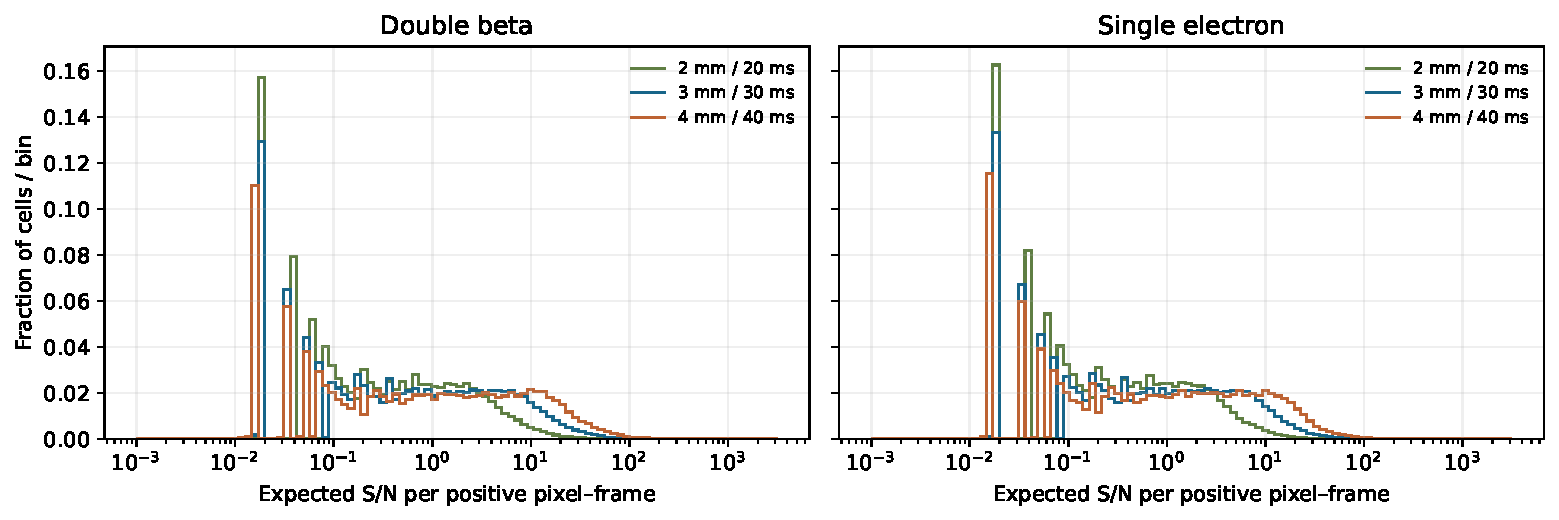
\includegraphics[width=\linewidth]{pilot_snr.pdf}
\caption{Expected S/N distributions from the saved corrected pilots. Every
positive input pixel--frame cell contributes. The plotted bins use a
logarithmic S/N axis; nonpositive values remain in the saved results.}
\label{fig:snr}
\end{figure}

The 2 mm configuration has been set aside for the present design because of
its lower S/N. The remaining choice is between 3 and 4 mm. The coarser grid
collects more charge in each cell and improves S/N, while the finer grid
samples the track more closely. Track continuity and the endpoint blobs will
determine which gives the better reconstruction. S/N is a quality measure;
the pilot applies no S/N acceptance cut.

\subsection{Compression and total charge}

Compression is measured by comparing the noiseless CSA estimate with the
linear prediction for the same input. A local-loss flag requires the chosen
fractional loss and a deficit of at least one frame ENC. A pad history is
counted once when any positive-input bucket meets the criterion. An affected
event contains at least one such pad history.

The compression deficit and total-charge bias describe different quantities.
For event input $N_{\rm tot}=\sum_{p,n}N_{p,n}$, they are
\begin{align}
 D&=\frac{\sum_{N_{p,n}>0}
  \max(\widehat N^{\rm linear}_{p,n}-\widehat N^{\rm CSA}_{p,n},0)}{N_{\rm tot}},
 \label{eq:deficit}\\
 B&=\frac{\sum_{p,n}\widehat N^{\rm CSA}_{p,n}-N_{\rm tot}}{N_{\rm tot}}.
 \label{eq:bias}
\end{align}
The signed sum in $B$ includes quiet and recovery frames. Table~\ref{tab:charge}
also gives its mean and event-to-event standard deviation after sampled noise
is added.

\begin{table}[htbp]\centering\scriptsize
\caption{Mean event charge diagnostics. Local-loss events contain at least one
positive cell with $\geq50\%$ response loss and a deficit of at least one ENC.
The bias uses the signed total over all saved buckets. These flags identify
local distortion; the events are retained. Pitch is in mm.}
\label{tab:charge}
\input{\CsaGenerated charge.tex}
\end{table}

\begin{figure}[htbp]\centering
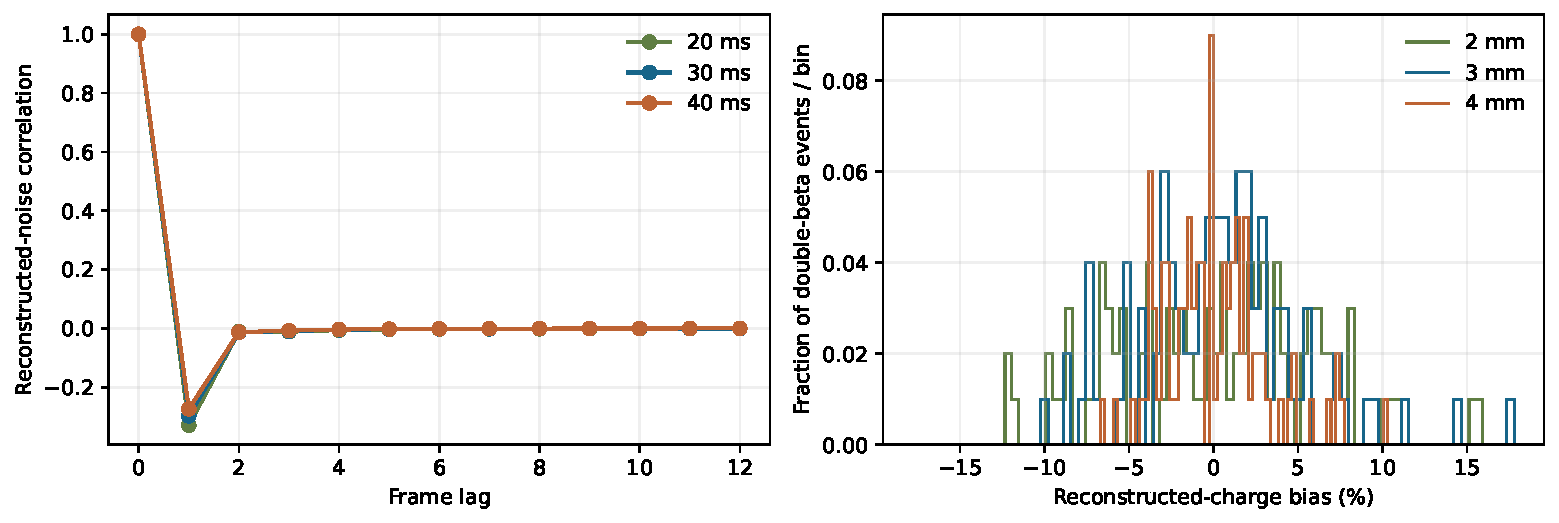
\includegraphics[width=\linewidth]{covariance_charge.pdf}
\caption{Left: temporal correlation of the reconstructed frame noise.
Right: signed total-charge bias after noise is added, for the selected
double-beta events.}
\label{fig:covariance}
\end{figure}
\begin{figure}[htbp]\centering
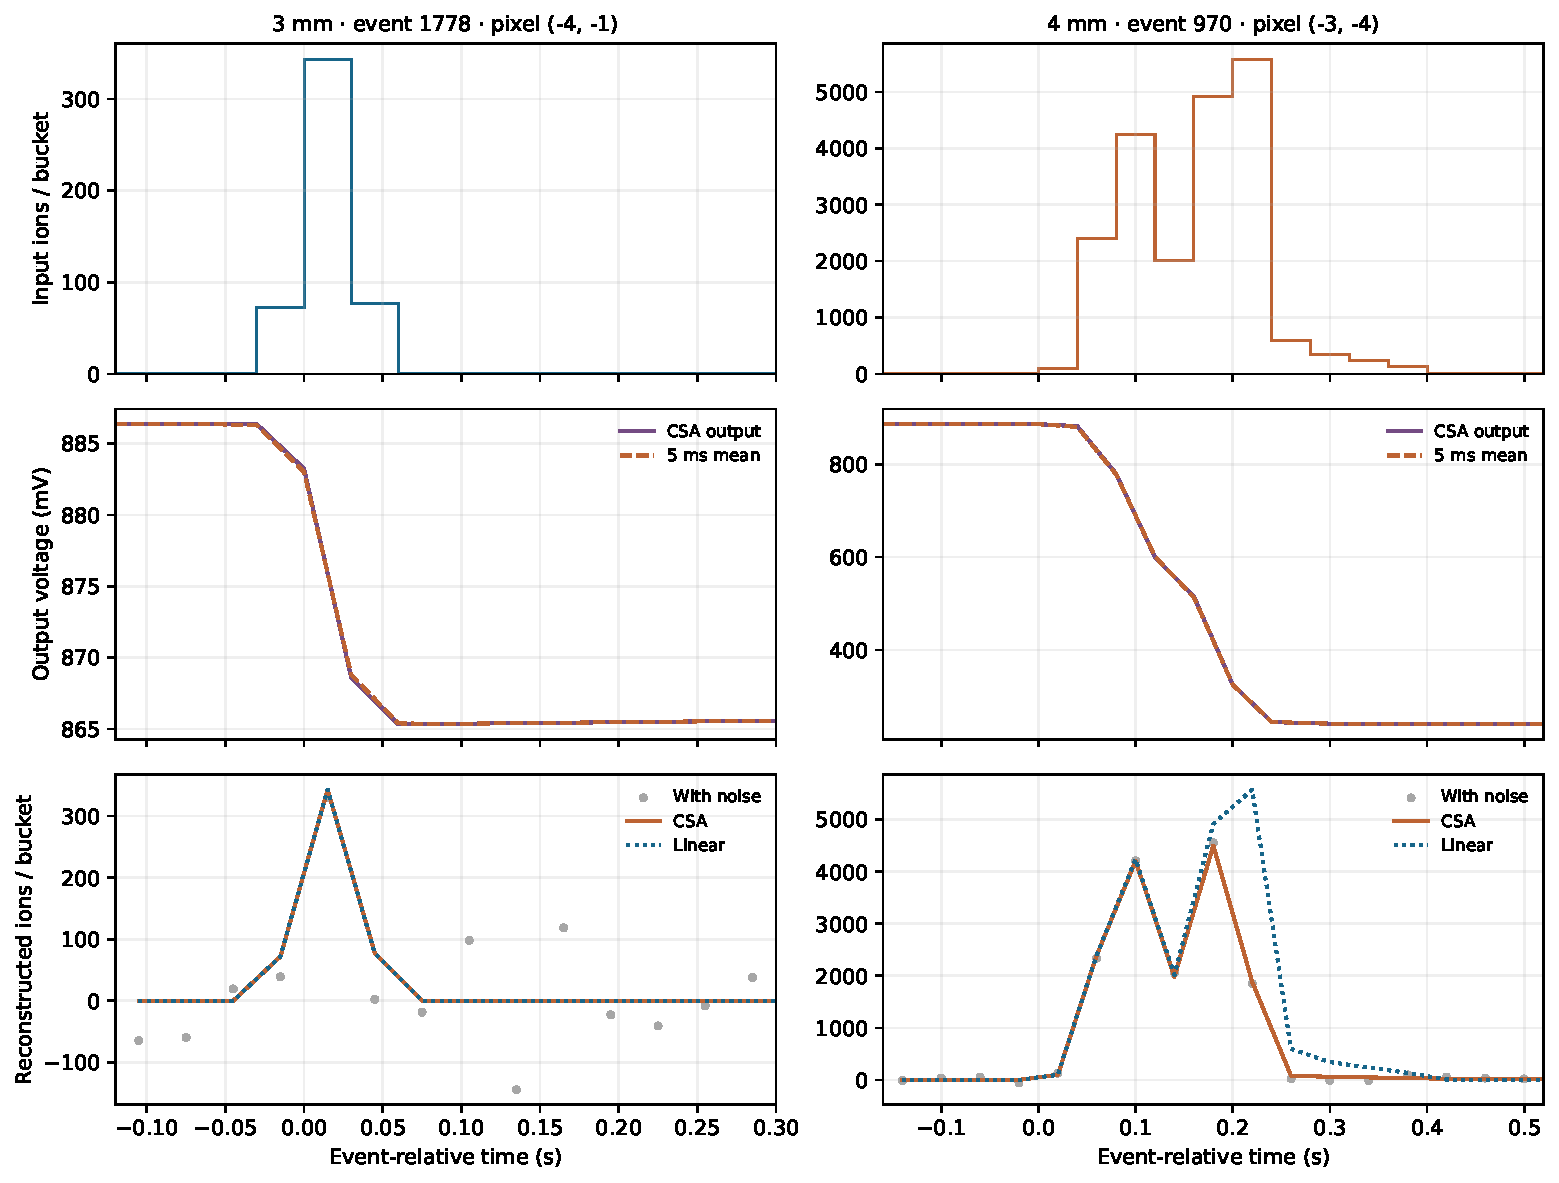
\includegraphics[width=\linewidth]{histories.pdf}
\caption{Examples from the saved double-beta pilots: a typical 3 mm history
(left) and a compressed 4 mm history (right). The rows show input counts,
CSA voltage and reconstructed counts. Empty buckets and the accumulated
voltage are included. The figures show the event interval; the files also
retain the recovery window.}
\label{fig:histories}
\end{figure}

\section{Saved reconstruction and numerical controls}

Each event is saved as a compact list of pixels with input charge, with a
complete time vector for every listed pixel. The matrix has one row per pixel
and one column per bucket in HDF5. Explicit pixel coordinates locate its rows;
they need not form a rectangular spatial grid. An isolated deposit far from
the main track adds its own pixels without adding the intervening pixels.

The output preserves input counts, the linear reference, the noiseless CSA
estimate, the noise realisation, the final reconstructed counts and the
voltage averages. Zero-input buckets within these histories and signed
reconstructed values are retained. Absent pixels received no input charge;
their electronic noise was not simulated. Measured zero suppression can be
studied later using the saved signals and an explicitly defined readout area.

Every response records the original event IDs, signed pixel and bucket
indices, geometry, event placement, input-file hash, circuit and reconstruction
cards, calibration, implementation identity and noise seeds. HDF5 files are
written atomically and marked complete after the requested events and ion
ledgers pass validation.

\begin{table}[htbp]\centering\small
\caption{Numerical response controls after reconstruction. Errors are measured
relative to the corresponding frame ENC.}
\label{tab:validation}
\input{\CsaGenerated validation.tex}
\end{table}

The note reduction checks \CsaNoteChecks\ matched-input and summary conditions,
including identical event IDs and primary-ion counts across geometries.
Additional checks cover the input-current integral, spectral quadrature,
covariance convergence and positive definiteness, noise sampling, frame
alignment, exact input-ion accounting, and Float32 output precision against
Float64 calculations. Each event begins at the quiescent operating point;
charge accumulated in preceding unrelated events is a separate operating
condition.

\appendix
\section{Covariance and noise sampling}

Equation~\eqref{eq:covariance} gives a Toeplitz covariance before the inverse,
with entries $(C_y)_{ij}=C_y(|i-j|)$. A Cholesky factor $L$ gives a noise
realisation $\boldsymbol\eta=L\mathbf z$, with independent standard-normal
components in $\mathbf z$. The stored reconstructed noise is
$M^{-1}\boldsymbol\eta$. Its covariance is Eq.~\eqref{eq:enc}.
The finite history and the quiet boundary frames make the final frame
variances slightly position dependent; the analysis uses those variances.

The covariance integration uses the saved one-sided spectrum. High-frequency
truncation for off-diagonal terms is accepted only when the omitted variance
bounds the covariance error within the configured tolerance. The diagonal
retains the full noise-band integral. Independent quadrature and zero-input
noise samples validate the resulting matrices.

\section{Reproducing the note}

The calculation follows the repository workflow: Julia performs the numerical
reduction and writes HDF5; Python produces the tables, macros and figures.
The note card is \texttt{config/specs/runs/csa\_design\_note.toml}.
It selects the completed corrected pilot indexes and the saved retention scan.
From the repository root, using the project's Julia scientific depot:
\begin{verbatim}
julia --project=. scripts/production/reduce_csa_design.jl
work/event-viewer-venv/bin/python \
  scripts/production/present_csa_design.py
\end{verbatim}
The numerical summary and source hashes are saved in
\texttt{results/csa\_design/}. Generated tables, values, figures and a standalone
copy of this source are in \texttt{latex\_generated/csa\_design/}.
Presentation can be regenerated from the saved summary alone.

Each pilot has a run card and a reconstruction card. For example, the 2 mm
calculation is reproduced with
\begin{verbatim}
work/event-viewer-venv/bin/python \
  scripts/production/run_ion_csa_pilot.py \
  --config config/specs/runs/ion_csa_v3_pilot_2mm.toml
work/event-viewer-venv/bin/python \
  scripts/production/run_ion_csa_correction.py \
  --config config/specs/runs/ion_csa_v3_corrected_pilot_2mm.toml
\end{verbatim}
The corresponding 3 and 4 mm cards select their saved inputs. The production
entry point gathers the six corrected pilot responses under the common run
card and writes their manifests:
\begin{verbatim}
julia --project=. scripts/production/run_ion_csa.jl \
  config/specs/runs/ion_csa_v3_pilot_all.toml
\end{verbatim}
The production schema is \texttt{nausicaa.ion\_csa\_response.v1}.
\texttt{read\_event} in \texttt{src/ion\_signal/ion\_csa\_pipeline.jl}
returns an owned \texttt{ReconstructedIonEvent}, with input, mean, noise and
reconstructed matrices indexed by (frame, pad) in Julia. The physical HDF5
axes are (pad, frame); the covariance reader supplies the matching frame
covariance. The output metadata records the input-based channel selection
and the treatment of absent pixels.

The companion HTML displays provide individual histories, severity selectors,
distributions and numerical controls. Large HDF5 and simulation waveforms remain outside
Git; the scripts, cards, source manifests and report artifacts are tracked.

\bibliographystyle{unsrtnat}
\IfFileExists{references.bib}{\bibliography{references}}{\bibliography{../../notes/physics/references}}
\end{document}
